\begin{problem}{별자리}
	{standard input}{standard output}
	{1초}{64MB}{}
	
	JOI 군은 별이 빛나는 밤하늘을 관찰하는 것을 사랑하는 소년이다. 매일 밤 밤하늘을 관찰해서, 각각 별이 어느 별자리에 속하는지 알아보는 것을 즐기고 있다.
	
	어느 날 밤 JOI 군은 밤하늘을 관찰하면서 본 적 없는 별을 $N$ 개 발견했다. 이 별이 어느 별자리에 위치하는지 신경 쓰인 JOI 군은 밤하늘의 사진을 찍어서 다음날 도서관에서 이 별들에 대해 조사했고, 이 별은 모두 별자리 A나 별자리 B에 속한다는 것과 이 별 중 몇 개가 어느 쪽의 별자리에 속하는지 알았다. 하지만, 그 이외의 별에 대해서는 어느 별자리에 속하는지 몰랐다. JOI 군은 별자리 A와 별자리 B를 구성하는 별의 집합으로 가능한 것이 몇 가지 있는지 궁금해졌다. 덧붙여서, 별의 크기는 매우 작으므로 점으로 봐도 좋다.
	
	단, 별자리는 사진에 있는 한 개 이상의 별과 별 두 개를 잇는 선분 몇 개로 되어있고, 다음 조건을 만족한다. 별이 한 개만 있는 것도 올바른 별자리인 것에 주의하여라.
	
	\begin{itemize}
		\item 어떤 별자리에 속한 두 개의 별은, 사진에 있는 그 별자리에 속한 선분을 통해 서로 도달할 수 있다.
		\item 어떤 별자리에 속한 선분과 다른 별자리에 속한 선분은 서로 교차하지 않는다.
	\end{itemize}
	
	또한, JOI 군이 발견한 별들은 다음의 조건을 만족한다.
	
	\begin{itemize}
		\item 어떤 세 개의 별도, 사진에서 일직선 상에 존재하지 않는다.
		\item 모든 별은 별자리 A 혹은 별자리 B에 속하며, JOI 군이 발견한 별 이외에 별자리 A 또는 별자리 B에 속하는 별은 존재하지 않는다.
	\end{itemize}
	
	$N$ 개의 별의 정보가 주어졌을 때, 별자리 A와 별자리 B를 구성하는 별의 집합으로 가능한 경우의 수를 $1\ 000\ 000\ 007 (=10^9 + 7)$로 나눈 나머지를 구하는 프로그램을 작성하여라.
	
	\Constraints
	
	
	\begin{tabular}{ll}
		$2 \le N \le 100\ 000$ & JOI 군이 발견한 별의 수 \\
		$0 \le X_i \le 10^9$, $0 \le Y_i \le 10^9$  & 	$i$ 번째 별의 사진에서의 위치 \\
	\end{tabular}
	
	
	\InputFile
	
	다음 정보가 표준 입력으로 주어진다.
	
	\begin{itemize}
		\item 첫째 줄에는 정수 $N$이 주어지며, JOI 군이 발견한 별의 수를 의미한다.
		\item 다음 $N$ 개의 줄에는, 별의 정보가 주어진다. $i+1$ ($1 \le i \le N$) 번째 줄에는, 세 개의 정수 $X_i$, $Y_i$, $C_i$가 공백으로 구분되어 주어진다. $X_i$, $Y_i$는 $i$ 번째 별의 사진에서의 위치가 $(X_i, Y_i)$라는 것을 의미한다. $C_i$는 별 $i$가 별자리 A와 별자리 B 중 하나에 속해있다는 것을 의미한다.
		\begin{itemize}
			\item $C_i=0$인 경우, $i$ 번째 별이 어느 별자리에 속해 있는지 모른다는 것을 의미한다.
			\item $C_i=1$인 경우, $i$ 번째 별이 별자리 A에 속해 있다는 것을 의미한다.
			\item $C_i=2$인 경우, $i$ 번째 별이 별자리 B에 속해 있다는 것을 의미한다.
		\end{itemize}
	\end{itemize}
	
	
	\OutputFile
	
	별자리 A와 별자리 B를 구성하는 별의 집합으로 가능한 경우의 수를 $1\ 000\ 000\ 007 (=10^9 + 7)$로 나눈 나머지를 첫째 줄에 출력하여라. 그런 별의 집합이 존재하지 않을 경우, 0을 출력하여라.
	
	\Scoring
	
	채점 데이터 중, 배점의 10\%에 대해 $N \le 10$을 만족한다.
	
	채점 데이터 중, 배점의 50\%에 대해 $N \le 300$을 만족한다.
	
	\Examples
	
	\begin{example}
		\exmp{
			4
			1 1 1
			2 1 1
			1 2 0
			2 2 2
		}{%
			2
		}%
	\end{example}
	
	이 입력 예제는 다음의 그림에 대응된다. 검은색 점이 별자리 A를 구성하는 별들이고, 하얀색 점이 별자리 B를 구성하는 별들이며, $\times$표시는 어떤 별자리에 속하는지 모르는 별이다.
	
	\begin{center}
	\begin{tabular}{cc}	
	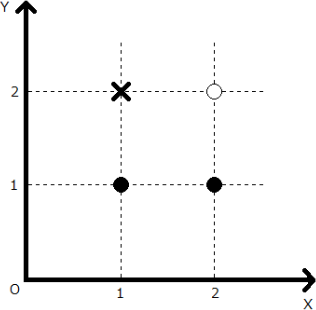
\includegraphics[width=0.4\linewidth]{img1.png} &  \hspace{0.45\linewidth} \\
	\end{tabular}
	\end{center}
	
	
	
	이 입력 예제에 대응하는 답은 3번 별이 별자리 A에 포함되는 경우와 별자리 B에 포함되는 경우 두 가지가 있으며, 각각의 경우 별자리 그림은 다음과 같다. 3번 별이 A에 포함되는 경우, 별자리 A의 선분을 그리는 방법이 여러 종류가 있지만 모두 한 종류로 셈에 주의하여라.
	
	\begin{center}
	\begin{tabular}{cc}	
		3번 별이 별자리 A에 포함되는 경우 & 3번 별이 별자리 B에 포함되는 경우 \\
		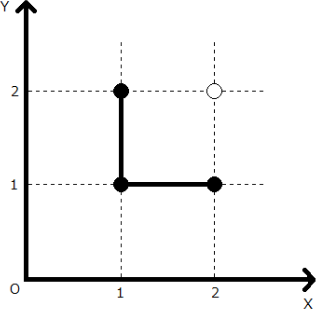
\includegraphics[width=0.4\linewidth]{img2.png} & 	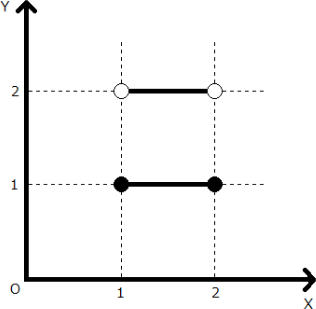
\includegraphics[width=0.4\linewidth]{img3.png} \\
	\end{tabular}
	\end{center}


\end{problem}

